\documentclass[titlepage]{article}
\usepackage{graphicx} % Required for inserting images

\title{final\_cw}
\author{Arash Amiri}
\date{Bhman 1403}

\begin{document}

\maketitle
\tableofcontents
\newpage
\section{Git and Github}
\subsection{Repository Initialization and Commits}
like every normal person i opened github website, then i clicked on \textit{make a new repository} bottom and put a name for that and then i was done!
\subsection{cloning}
after i generated a repository i had to clone it in my local machine! so i found it's html link in code section of my repository, and then i used the command \textbf{git clone \textit{my repository link}}. and it got done too
\section{Exploration Tasks}
\subsection{Vim Advanced Features}
\begin{enumerate}
    \item Recording and Replaying actions\newline
    by entering (q) in normal mode and then a key character such as (a) we can record some actions and then by entering (q) we stop recording and by (@<key character>) that actions replay again!
    \item Clipboard Management\newline
    by typing ("<some key character>y) the selected area by visual mode gets copied in that key character and whenever we like we can paist it by ("<key character>p)
    \item folding\newline
    in vim (Normal mode) by zM all sections get closed, zR opens them
\end{enumerate}
\subsection{Memory profiling}
\subsubsection{Memory Leak}
memory leak happens when we use memory to initialize some variables in our program but they don't get free after program is finished. some functions can cause this problem such as malloc() in c
\subsubsection{Memory profilers}
Valgrind is a tool to solve the memory leak problem! it checks if program has used some special functions which can unfree memory and free that space! it also finds accebility of user to some space of memory which user didn't suppose to access
\subsection{GNU/Linux Bash Scripting}
\subsubsection{fzf}
it is a powerful command line tool which help us search folders, files, history commands and ...!it is so powerful and you don't need to search exact name of your purpused item! it finds every algorithms and find your item by incompleted searches!\newline
underline{ls | fzf}:\newline
this command lists all the files and items in currient dir and we can search whatever we want there and it simply show us where it is!
\subsubsection{ Using fzf to find your favorite PDF}
\begin{enumerate}
    \item fd -e pdf
    \item fd -e pdf | fzf
\end{enumerate}
\subsubsection{Opening the file using Zathura}
zathura \$(find /path/to/search -name "filename.pdf")
\section{Git and FOSS}
\begin{figure}[h]
    \centering
    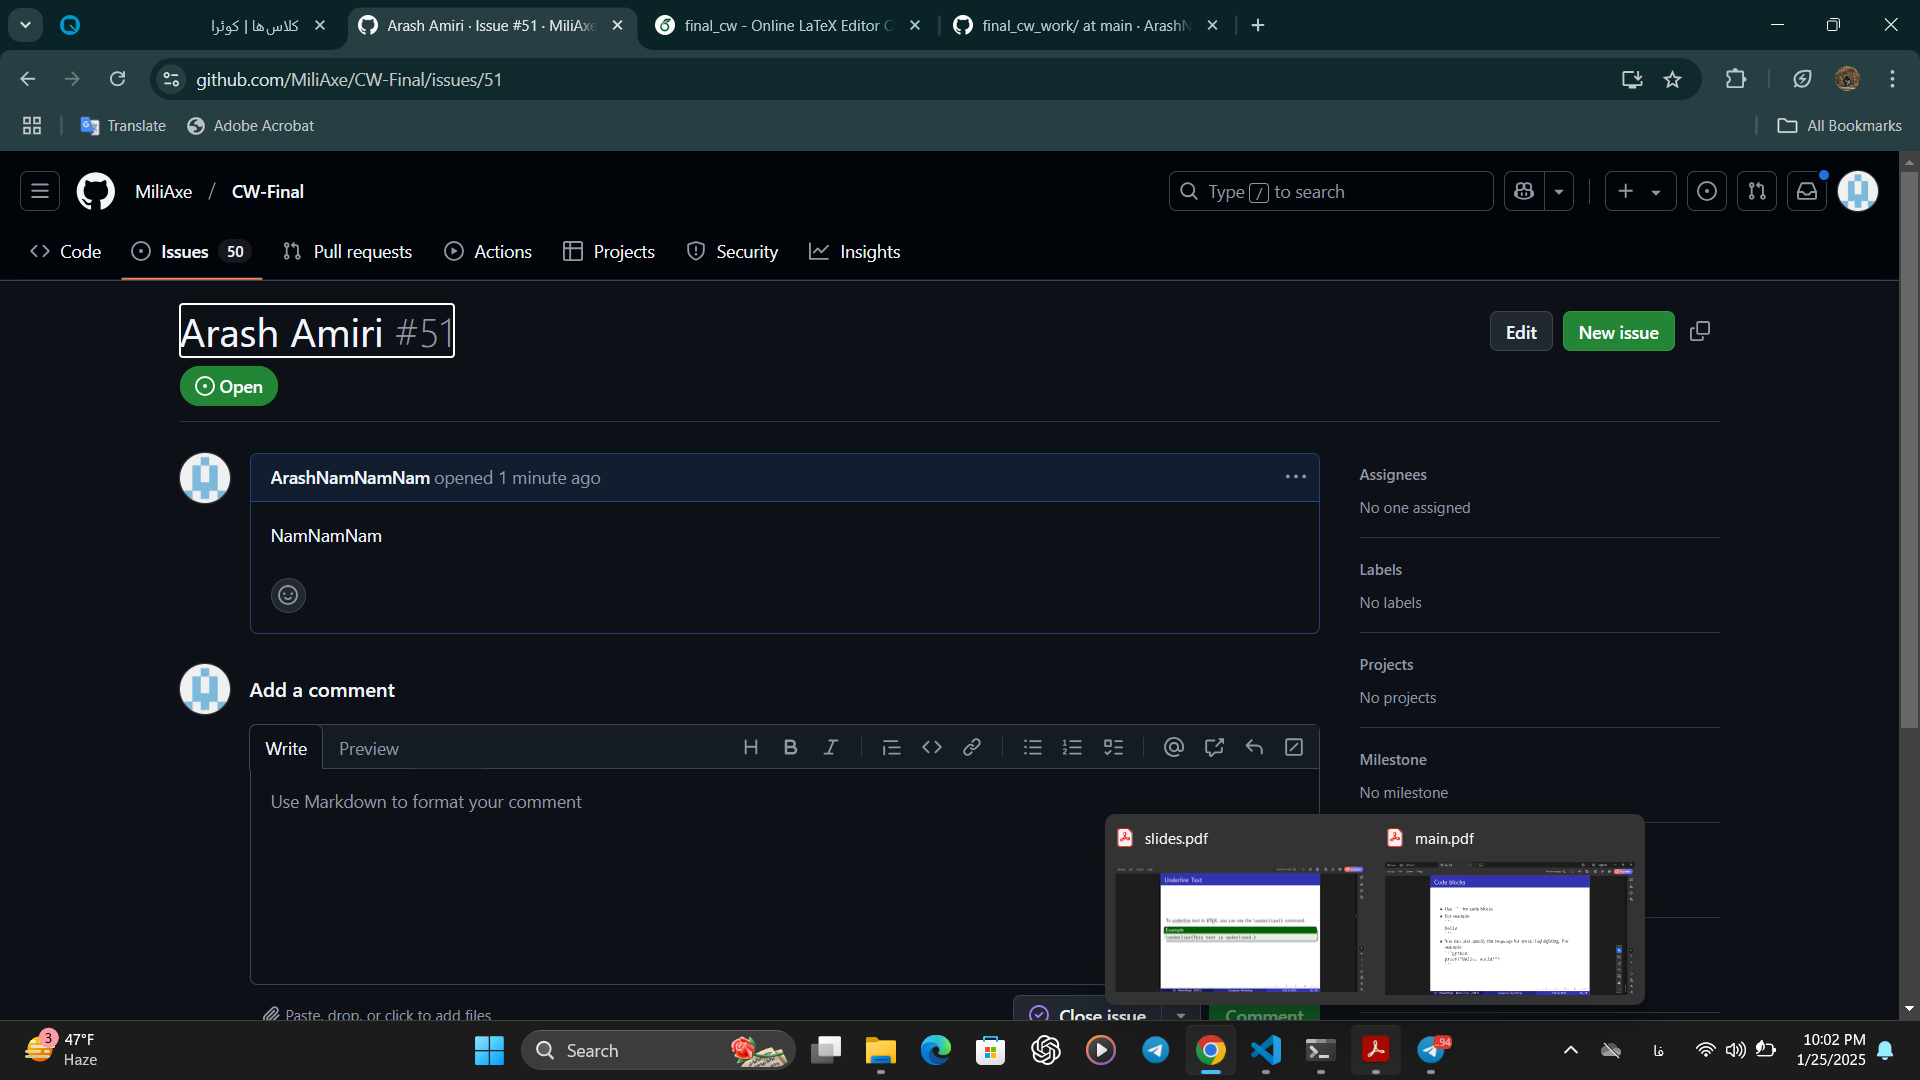
\includegraphics[width=0.5\textwidth]{image.png}
    \caption{here is my smple issue}
\end{figure}
\section*{FOSS contribution}
actually it seems fun to do project in some FOSS environments such as github! and i love teamwork. so yes i do see myself in such a position!
\end{document}
